%\begin{itemize} 
%\item{ }
%A brief textual description of the overall flow diagram (along with its functional operation in the different user scenarios described in the first stage of the project).
%\item{ }
%A specification of each algorithm and associated data structures together with its entities, attributes, and operations ( include an English description of how they relate to your user scenario(s)).

%\end{itemize}

\begin{itemize} 
\item{  Short Textual Project Description. }

Here, for conveniently understanding and evaluating our project, a recommendation system for users who are in demand of public services, like restaurants, pet shops, or grocery stores, is illustrated as an example. From our Yelp Dataset, as mentioned above, we extract three key factors, including user's ratings, the category of a business unit and its attributes (i.e. prices for different foods, alcohol provider or not, payment ways, Wi-Fi service, good for group food or not, good for kids or not, easy-appointment access, reservation time and wheelchair, etc.). The relative information between these entities (users and business unit) shows as graph edge weights in our algorithm, and will be calculated using users' ratings. When executing our recommendation system, an optimal recommendation list will be generated based on built-in grading function; and the recommendation list is composed of a set of users and business unit with some specific relationship. For examples, a list of restaurants are rated about the same within a certain set of users.\\


Flow diagram textual description:\\


1. Obtain raw dataset and collect the clean data satisfying the requirement for the further analysis using the procedure ``BUILD\_GRAP\_LIST", where the user, business units (business company) information and corresponding review (e.g. restaurant ratings) are collected and finally form an adjacent list for these information.

2. Build up the objective graph using three procedures: BUILD\_FIRST\_LAYER, BUILD\_SECOND\_LAYER and BUILD\_THIRD\_LAYER. Inside the objective graph, the edges weights between nodes in different definition layers (users and business units) are generated based on our specifically-designed algorithms. collaborative filtering; content based.

3. Generate a recommendation list with the procedure ``FORM\_REC\_LIST" with providing an accuracy/quality rate from the procedure ``EVALUATE\_ACCURACY".

4. Evaluate different recommendation lists by modifying and improving the algorithm input parameters with corresponding accuracy/quality rates by repeating Step 1to 3.

5. Select the best recommendation list with the optimal accuracy/quality rate.\\

In our algorithm, the space complexity is individual\_node\_unit * \textit{O}(\textit{N} = numbers of users and business units). Because the multiple pointers exist (i.e. a user can rate a lot of business units), individual\_node\_unit can be considered to use two ways: i) an adjacent list to preserve these points (PROS: minimize the space complexity; CONS: increase the algorithm complexity when building up the objective graph); i) an adjacent matrix (PROS: easy to access and build up an objective; CONS: have huge waste in space if the maximum rating number is very high and few users have provided multiple rating in different business units). We need to build up the objective graph and search the entire graph, based on different implementation methods, the optimal time complexity in our recommendation system is \textit{O}(\textit{E}*log(\textit{N})) $ \approx $ \textit{O}(\textit{N}*log(\textit{N}) (if multiple ratings are few), \textit{E} is the total edge.\\

\item{ Flow Diagram. }
\begin{figure}[h] \label{fig:flowDiag}
\begin{center}
    {\scalebox{0.3}{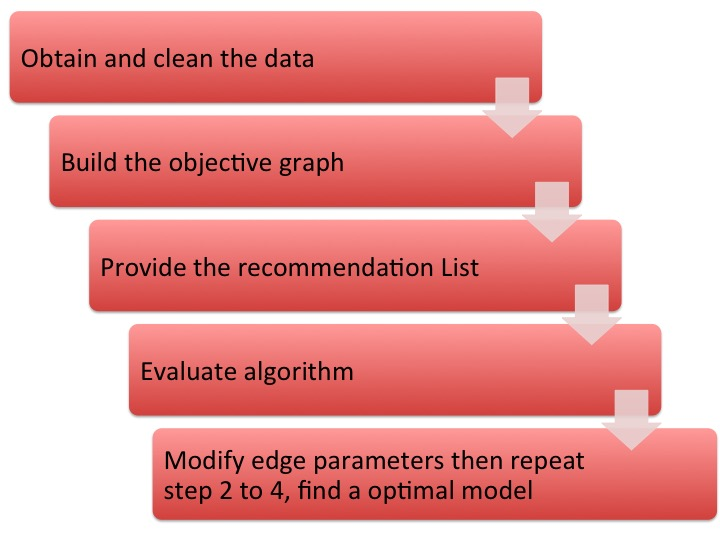
\includegraphics{FlowDiagram.jpg}}}
 \caption{Flow Diagram}
\end{center}
\end{figure}

\item{ High Level Pseudo Code System Description. }
\begin{algorithm}
\caption{Graph-based recommendation system}\label{algo-pseudo}
\begin{algorithmic}
\State Clean and import the data
%\State Partition dataset by user\_info, business\_info and view\_info, build the whole adjacent list of the graph by the clean dataset
\Procedure {Build\_Grap\_List}{}
    \State $\textit{user\_info} \gets \text{input user\_info}$
    \State $\textit{business\_info} \gets \text{input business\_info}$
    \State $\textit{review\_info} \gets \text{input review\_info}$
    \State $\textit{G\_list} \gets \text{build a adjacent graph list by the above dataset}$
\EndProcedure

\Statex

\State Build the objective graph
%\State Build the objective recommendation graph layer by layer (layer 0 is the objective node user A)

\Procedure{Build\_First\_Layer}{user node A, G\_list}
\State $\textit{find(first\_ln)} \gets \text{All nodes link to node A}$
    \ForAll {$node \in first\_ln$} 
          \State $node\_edge = RStar$ %\Comment {get edge from node A}
    \EndFor
\EndProcedure

\Procedure{Build\_second\_Layer}{\textit{first\_ln, G\_list}}
\State $\textit{find(second\_ln)} \gets \text{All nodes link to the first layer}$
    \ForAll {$node \in second\_ln$} 
          \State $node\_edge = RStar + RAve()$ %\Comment {get edge from nodes in first layer}
    \EndFor
\EndProcedure

\Procedure{Build\_third\_Layer}{\textit{first\_ln},\textit{second\_ln},G\_list}
\State $\textit{find(third\_ln)} \gets \text{All nodes link to nodes in second layer}$
    \ForAll {$node \in third\_ln$}
         \If {$node.cate \in set(first\_ln.cate)$}
                \State \textit{Aux(cate,attr) = Aux1(cate)+Aux(attr)}
         \Else
                \State \textit{Aux(cate,attr) = 0}
         \EndIf
    \EndFor                  
    \ForAll {$node \in third\_ln$} 
          \State $node\_edge = RStar + RAve()+ Aux(cate,attr)$ %\Comment {get edge from nodes in second layer}
    \EndFor
\EndProcedure

\Statex
\State Compute the longest path to each leaves and give the recommendation list

\Procedure {Form\_Rec\_List}{user node A, first\_ln, second\_ln, third\_ln}
    \State Rec\_List =\{\}
    \ForAll {$node \in third\_ln$}
         \State $node.lp() \gets \text{compute the longest path from node A} \hfill \break
         \text{\ \ \ \ \ \ \ \ \ \ \ \ \ \ \ \  \ \ \ \  \ \ \ \ by node.lp}$
    \EndFor
    Raw\_Rec\_List = sort(third\_ln) 
   \ForAll {$element \in Raw\_Rec\_List$}
         \If {$element \in first\_ln$}
                 \State do nothing
         \Else
                 \State Rec\_List.add(element)
         \EndIf
   \EndFor
\Return Rec\_List
\EndProcedure


\Statex
\State Provide the Accuracy Rate

\Procedure{Evaluate\_Accuracy}{}
    count = 0
    \For {$i \leftarrow 1 {\; \rm to\;} length(first\_ln)$}
            \If {$Raw\_Rec\_List[i] \in first\_ln$}
                     count +=1
            \EndIf
    \EndFor
\Return   Acc\_rate = count / length(first\_ln)        
\EndProcedure
\end{algorithmic}
\end{algorithm}

\item{Algorithms and Data Structures. }

Our algorithm design bases on such a basic idea: users who have similar taste in business units tend to review a specific business units with close score. Such a set of users should be a potential consumer group for some business units in a particular category. For example, finding out the people who love French cuisine is very meaningful if we can also recommend some good French restaurant to them. Thus, the first thing we do here is to correlate the similar patterns of users' rating from different business units; then we can recommend the favorite business units of a user to other users who have similar taste. 

The detailed contents and data structures of our algorithm pipeline are shown in ``Algorithm 1". In the part I - ``Clean and import the data", the raw data are provided and generated the specific data structure recording the ratings of each user for different restaurants: an adjacent list or an adjacent matrix for each user. In the part II - ``Build the objective graph", the users' rating data are built up as an objective graph data structure with specifically-designed edge weights by connecting users and business units with similar ratings, etc. In the part III - ``Compute the longest path to each leaves and give the recommendation list", we obtain list output using some algorithm similar to finding out the longest path in the directed acyclic graph (DAG). In the part IV - ``Provide the Accuracy Rate", a double floating value is provided by in order accessing each unit of the recommendation list from the part III.

\begin{figure}[h] \label{fig:representation_alg_1}
	\begin{center}
		\advance\rightskip-1cm
		{\scalebox{0.3}{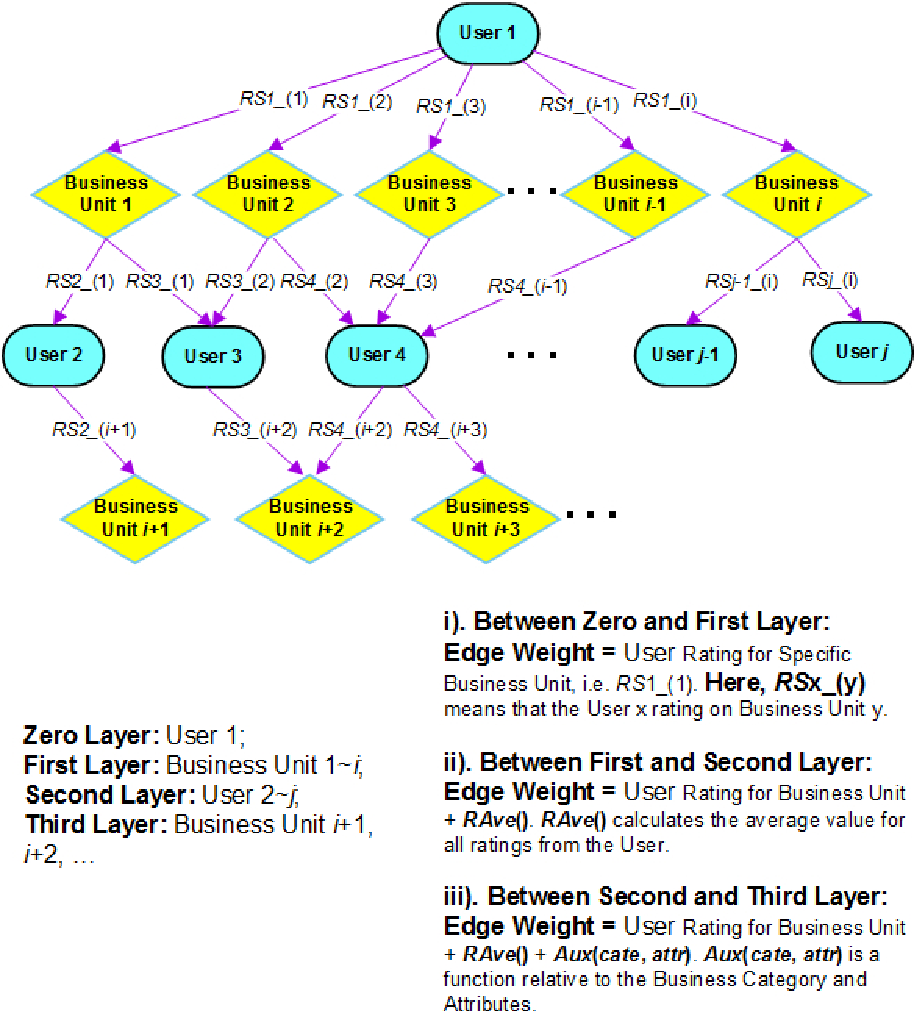
\includegraphics[width=300mm]{representation_alg_1.pdf}}}
		\caption{The objective graph representation in Algorithm 1}
	\end{center}
\end{figure}

\end{itemize}

\begin{itemize} 
\item{  Flow Diagram Major Constraints.}
\begin{itemize} 
\item{ Integrity Constraint. }
\\1. The input user need to have sufficient  reviews on record. Our recommendation system provides recommendation list by finding similar users based on input user's reviews. And it does so by comparing the reviews on business units that serve same purpose. The more reviews the input user has, the more accurate of measurement we have on its taste, and therefore, the better the recommendation can be.
\end{itemize}
%\begin{itemize} 
%Please repeat the pattern for each integrity constraint.
\end{itemize}
